\documentclass[a4paper]{article}

\usepackage[english]{babel}
\usepackage[utf8]{inputenc}
\usepackage{amsmath}
\usepackage{amsfonts}
\usepackage{graphicx}
\usepackage[colorinlistoftodos]{todonotes}

\title{Support Vector Machines}
\author{Bingyu Wang, Virgil Pavlu}
\date{\today}

\begin{document}
\maketitle
\section{What's SVM}
The original SVM algorithm was invented by Vladimir N. Vapnik\footnote{http://en.wikipedia.org/wiki/Vladimir\_Vapnik} and the current standard incarnation (soft margin) was proposed by Corinna Cortes\footnote{http://en.wikipedia.org/wiki/Corinna\_Cortes} and Vapnik in 1993 and published in 1995.

A support vector machine(SVM) constructs a hyperplane or set of hyperplanes in a high- or infinite-dimensional space, which can be used for classification, regression, or other tasks. Intuitively, a good separation is achieved by the hyperplane that has the largest distance to the nearest training data point of any class (so-called functional margin), since in general the larger the margin the lower the generalization error of the classifier.\footnote{http://en.wikipedia.org/wiki/Support\_vector\_machine} In this notes, we will explain the intuition and then get the primal problem, and how to translate the primal problem to dual problem. We will apply kernel trick and SMO algorithms to solve the dual problem and get the hyperplane we want to separate the dataset.
Give general idea about SVM and introduce the goal of this notes, what kind of problems and knowledge will be covered by this node. 

In this note, one single SVM model is for two labels classification, whose label is $y \in \{-1, 1\}$. And the hyperplane we want to find to separate the two classes dataset is $h$, for which classifier, we use parameters $w, b$ and we write our classifier as
$$
h_{w,b}(x) = g(w^T x + b)
$$

Here, $g(z) = 1$ if $z \geq 0$, and $g(z) = -1$ otherwise. 

\section{Margins}

Following Andrew Ng\footnote{CS229 Lecture notes, Part V Support Vector Machines}, we will start the by talking about margins, which can give us the ``confidence'' of our predictions.

Consider logistic regression, where the probability $p(y = 1 | x; w)$ is modeled by $h_w(x) = g(w^T x)$.We would then predict ``1" on an input $x$ if and only if $h_w(x) \geq 0.5$, or equivalently, if and only if $w^T x \geq 0$. Consider a positive training example $(y = 1)$. The larger $w^T x$ is, the larger also is $h_w(x) = p(y=1 | x; w, b)$, and thus also the higher our degree of ``confidence" that the label is 1. Thus informally we can think of our prediction as being a very confident one that $y = 1$ if $w^T x \gg 0$. Similarly, we think of logistic regression as making a very confident prediction of $y = 0$, if $w^T x \ll 0$. Given a training set, again informally it seems that we'd have found a good fit to the training data if we can find $w$ so that $w^Tx_i \gg 0$ whenever $y_i = 1$, and $w^T x_i \ll 0$ whenever $y_i = 0$, since this would reflect a very confident (and correct) set of classifications for all the training examples. This seems to be a nice goal to aim for, and we?ll soon formalize this idea using the notion of functional margins. 

For a different type of intuition, consider the following Figure \ref{fig:confident}, in which x's represent positive training examples, o's denote negative training examples, a decision boundary (this is the line given by the equation $w^Tx  = 0$, and is also called the \textbf{separating hyperplane}) is also shown, and three points have also been labeled A, B and C.
\begin{figure}[h!]
  \centering
    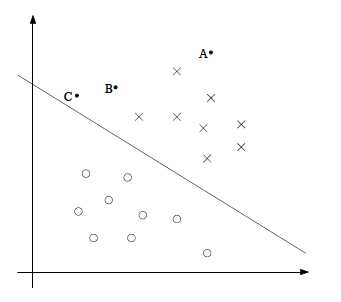
\includegraphics[width=0.5\textwidth]{./images/confident}
  \caption{Confident Example, linearly separable.}\label{fig:confident}
\end{figure}

Notice that the point A is very far from the decision boundary. If we are asked to make a prediction for the value of $y$ at A, it seems we should be quite confident that $y=1$ there. Conversely, the point C is very close to the decision boundary, and while it's on the side of the decision boundary on which we would predict $y = 1$, it seems likely that just a small change to the decision boundary could easily have caused our prediction to be $y = 0$. Hence, we're much more confident about our prediction at A than at C. The point B lies in-between these two cases, and more broadly, we see that if a point is far from the separating hyperplane, then we may be significantly more confident in our predictions. Again, informally we think it'd be nice if, given a training set, we manage to find a decision boundary that allows us to make all correct and confident (meaning far from the decision boundary) predictions on the training examples. 

In another word, if we could find a decision boundary, who can give us a larger margin, it will be better than the one give us a smaller margin. From the following Figure \ref{fig:margin}, we can tell that the black decision boundary is better than the green decision boundary, because the black one gives us a larger margin than the green one.
\begin{figure}[h!]
  \centering
    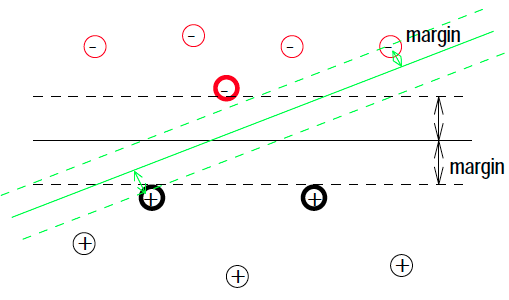
\includegraphics[width=0.8\textwidth]{./images/margin}
  \caption{Margin Example. The black separating plane is better than the green one, because it has larger margins (sits more ``in the middle''). A mechanical analogy: if the separating plane is free to rotate but constrained to be separator, when the points start pushing force towards the plane, the plane will settle in an equilibrium ``middle'' position - thats where the black separator is. }\label{fig:margin}
\end{figure}


\subsection{Functional and Geometric Margins}
Lets now formalize the margin intuition into  notions of the functional and geometric margins. Given a training example ($x_i$, $y_i$), we define the functional margin of (w, b) with respect to the training example
$$
	\hat{\gamma}_i = y_i (w^T x + b)
$$

Note that if $y_i = 1$, then for the functional margin to be large (i.e., for our prediction to be confident and correct), we need $w^T x + b$ to be a large positive number. Conversely, if $y_i = -1$, then for the functional margin to be large, we need $w^T x + b$ to be a large negative number. Moreover, if $y_i (w^T x + b) > 0$, then our prediction on this example (x\_i, y\_i) is correct. Hence, a large functional margin represents a confident and a correct prediction. 

Given a training set $S = \{(x\_i, y\_i); i = 1, 2, \dots, m\}$, we also define the function margin of $(w, b)$ with respect to S to be the smallest of the functional margins of the individual training examples. Denoted by $\hat{\gamma}$, this can therefore be written: 
$$
	\hat{\gamma} = \min_{i=1,\dots,m} \hat{\gamma}_{(i)} 
$$

Functional margins can represent a confident and a correct prediction. The larger functional margins, the classifier better. However, by scaling $w, b$, we can make the functional margin arbitrarily large without really changing anything meaningful. Typically for a linear classifier, the final prediction is made by applying the sign function $g$ to the linear score: 
	\[ g(z) = \left\{ 
  		\begin{array}{l l}
    			1 & \quad \text{if $z \geq 0$}\\
 			-1 & \quad \text{if $z < 0 $}
 		 \end{array} \right.\]
		 
We note for any scalar $c$ we can replace $w$ with $cw$ and $b$ with $cb$, and have that $g(w^Tx + b ) = g(cw^Tx + cb)$, this would not change the prediction $h_{w,b}(x) = g$ at all. I.e., g, and hence also $h_{w,b}(x)$, depends only one the sign, but not on the magnitude of $w^T + b$. However, replacing $(w,b)$ with $(cw, cb)$ also results in multiplying our functional margin by a factor of $c$. Thus, it seems that by exploiting our freedom to scale $w$ and $b$, we can make the functional margin arbitrarily large without really changing anything meaningful. We can make a reference decision on scale, and will choose the scale such that minimum functional margin is  $y(w^Tx + b)=1$.
% Intuitively, it might therefore make sense to impose some sort of normalization condition such as that $||w|| = 1$; i.e., we might replace $(w, b)$ with $(w/||w||, b/||w||)$, which can be solved by geometric margins.

\subsubsection{Geometric Margins}
In Figure \ref{fig:geometric}, the decision boundary corresponding to $(w, b)$ is shown, along with the vector $w$. Note that $w$ is orthogonal to the separating hyperplane.\footnote{http://mathworld.wolfram.com/NormalVector.html}. Consider the opposing points at $x_1$ and $x_2$ which represents training examples closest to each other with labels $y_1 = 1$, $y_2 = -1$. The distance to the decision boundary, or the geometric margin $\rho$, is half of line segment $x_1x_2$, one minimum margin on each side.  

\begin{figure}[t!]
  \hspace{-10ex}
    \includegraphics[width=1.2\textwidth]{images/svm_margin}
  \caption{Geometric Margin: $w$ and $b$ are scaled such that closest points are on the line $|w^Tx+b|=1$. If the plane is in the middle, the minimum margin (geometrical distance from plane to points) is $\rho = 1/w$. }\label{fig:geometric}
\end{figure}

As the picture shows, we have scaled (by a constant) $w$ and $b$ such that the closest points are on the line $|w^Tx+b|=1$. This is a reference decision, and it can be done since any scalar $c$ applied to $w,b$ does not change the plane : $cw^Tx+cb=0$ is the same plane as $w^Tx+b=0$. We can write this constraint, that all points are no closer than lines $|w^Tx+b|=1$ (either side of the plane) by using the labels for signs: $y(w^Tx+b)\geq1$. In other words, the constraints state that all functional margins are at least 1.

From $w^Tx_1+b=1$ and $w^Tx_2+b=-1$ we have that $w^T(x_1-x_2)=2$; considering that $w$ and $x_1-x_2$ are parallel vectors, we obtain that $||x_1-x_2|| = 2 / ||w||$. Since $||x_1-x_2|| = 2\rho$, we obtain that the minimum geometric margin is $\rho = 1/||w||$. 

% How to calculate $\gamma_i$\footnote{http://mathworld.wolfram.com/Point\-PlaneDistance.html}? In fact, it's the distance from point to plane. According the Point-Plane Distance calculation, we can solve $\gamma_i$ as following:
% $$
% 	\gamma_i = \frac{w^T x_i + b}{||w||} = (\frac{w}{||w||})^T x_i + \frac{b}{||w||}
% $$
%
% This was worked out for the case of a positive training example at A in the Figure \ref{fig:geometric}, where being on the ``positive'' side of the decision boundary is good. More generally, we define the geometric margin of $(w, b)$ with respect to a training example $(x_i, y_i)$ to be
% $$
% 	 \gamma_{i} = y_{i}((\frac{w}{||w||})^T x_{i} + \frac{b}{||w||})
% $$
%
% Note that if $||w|| = 1$, then the functional margin equals the geometric margin, this thus gives us a way of relating these two different notions of margin. Also, the geometric margin is invariant to rescaling of the parameters; i.e., if we place $w$ with $2w$ and $b$ with $2b$, then the geometric margin does not change.
%
% Finally, given a training set $S = \{(x_i, y_i); i = 1, 2, \dots, m\}$, we also define the geometric margin of $(w, b)$ with respect to $S
% $ to be the smallest of the geometric margins on the individual training examples:
% $$
% 	\gamma = \min_{i=1,\dots,m} \gamma_{i}
% $$


%%%%%%%%%%%%%%%%%%%%%%%%%%%%%%%%%%%%%%%%%%%%%%%%%%%%%%%%%%%%%%%%%%%%%%%%%%%%%%%%%%%%%%%%%%%
\section{The Optimal Margin Classifier}
From the intuition of margins before, we try to find a decision boundary that maximizes the geometric margin, since this would reflect a very confident set of predictions on the training set and a good ``fit'' to the training data. Specifically, this will result in a classifier that separates the positive and the negative training examples with a ``gap'' (geometric margin).

For now, we will assume that we are given a training set that is linearly separable; i.e., that it is possible to separate the positive and negative examples using some separating hyperplane. How could we find the one that achieves the maximum geometric margin? We will pose the following optimization problem: maximize the margin  $\rho = 1/||w||$, such that all points are no closer (on either side) than $|w^Tx+b|=1$ to the separating plane given by $w^Tx+b=0$; thus the constraints reflect our reference choice for scale. Since the labels are the same as the 1,-1 sides of the plane, we can rewrite the constraints as $y(w^Tx+b)\geq1$ for all training points $x$ with label $y\in \{-1,1\}$ (will have one constraint for each training point).



% \begin{align*}
% &\quad  \max_{\gamma, w, b} \gamma \\
% &\quad  \text{s.t.} \quad  y_{i}(w^Tx_{i} + b) \geq \hat{\gamma}, \quad i = 1, \dots, m \\
% &\quad   \quad \quad ||w|| = 1
% \end{align*}
%
% I.e., we want to maximize $\gamma$, subject to each training example having functional margin at least $\hat{\gamma}$. The $||w|| = 1$ constraint moreover ensures that the functional margin equals to the geometric margin, so we are also guaranteed that all the geometric margins are at least $\gamma$. Thus solving this problem will result in $(w, b)$ with the largest possible geometric margin with respect to the training set.
%
% If we could solve the optimization  problem above, we'd be done. But the ``$||w|| = 1$'' constraint is a nasty (non-convect) one, and this problem certainly is not in nay format that we can plug into standard optimization software to solve. So, let's try transforming the problem into a nicer one. Since we know that $\gamma = \frac{\hat{\gamma}}{||w||}$, so we can consider:
% \begin{align*}
% 	& \max_{\hat{\gamma}, w, b} \frac{\hat{\gamma}}{||w||} \\
% 	\quad & \text{s.t.} \quad y_i (w^T x_i + b) \geq \hat{\gamma}, \quad i = 1, \dots, m
% \end{align*}
%
% Here, we're going to maximize $\hat{\gamma}/||w||$, subject to the functional margins all being at least $\hat{\gamma}$. Moreover, we've gotten rid of the constraint $||w|| = 1$ that we didn't like. The downside is that we now have a nasty (non-convex) objective $\frac{\hat{\gamma}}{||w||}$; and, we still don't have any good solutions in this form of an optimization problem.
%
% If we keep going. Recall our earlier discussion that we can add an arbitrary scaling constraint on $w$ and $b$ without changing anything. This is the key idea we will use. We will introduce the scaling constraint that the functional margin of $w, b$ with respect to the training set must be 1:
% $$
% 	\hat{\gamma} = 1
% $$
% Since multiplying $w$ and $b$ by some constant results in the functional margin being multiplied by that same constant. So if now we set $\hat{\gamma} = 1$, we derive the formula as following:
% \begin{align*}
% 	 &\max_{\hat{\gamma}, w, b} \frac{\hat{\gamma}}{||w||} \\
% 	\Leftrightarrow & \max_{w, b} \frac{1}{||w||} \\
% 	\Leftrightarrow & \min_{w, b} ||w|| \\
% 	\Leftrightarrow & \min_{w, b} \frac{1}{2} ||w||^2
% \end{align*}

To make the math nicer we write the objective in terms of $||w||^2$, and we get the following optimization problem:\\

\textbf{SVM-PRIMAL OPTIMIZATION PROBLEM}\\
\begin{align}
	& \min_{w, b} \frac{1}{2} ||w||^2 \\
	\quad & \text{s.t.} \quad y_i (w^T x_i + b) \geq 1, \quad i = 1, \dots, m
\end{align}

We've now transformed the problem into a form that can be efficiently solved. The above is an optimization problem with a \textbf{convex quadratic objective (1)} and only \textbf{linear constraints (2)}. Its solution gives us the optimal margin classifier. This optimization problem can be solved using commercial quadratic programming(QP) code\footnote{http://en.wikipedia.org/wiki/Quadratic\_programming} or (better) with duality formulation. 

We will use Lagrange duality to solve the above constrained convex optimization problem. This will allow the use kernels, and it is also more efficient. 




%%%%%%%%%%%%%%%%%%%%%%%%%%%%%%%%%%%%%%%%%%%%%%%%%%%%%%%%%%%%%%%%%%%%%%%%%%%%%%%%%%%%%%%%%%%%%%%
\section{Solution part 1: the dual problem}
In this section, we need apply the duality mentioned above to transform the original problems to a easier problem, which can be solved by SMO algorithm, talk about it later. First, we derive the process from original problem to dual problem on separable case and later we will work on the non-separable case. We will show how the dual problem is written in Lagrangian variables $\alpha, \beta$, and that $w, b$ are a function of these dual variables (and the data).

\subsection{Linearly Separable case}
The separable case means the training dataset can be separated by one line, which is shown in Figure \ref{fig:separable}. 
\begin{figure}[h!]
  \centering
    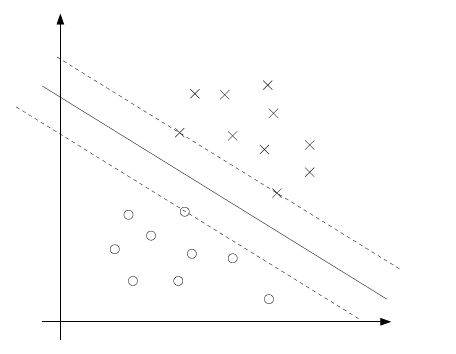
\includegraphics[width=0.7\textwidth]{./images/separable}
  \caption{Seperable Example}\label{fig:separable}
\end{figure}
We will starts from the original problem:

\textbf{SVM-PRIMAL problem}
\begin{align*}
	& \min_{w, b} \frac{1}{2} ||w||^2 \\
	\quad & \text{s.t.} \quad y_i (w^T x_i + b) \geq 1, \quad i = 1, \dots, m
\end{align*}

We will first transform the constraints to standard form, and write down the Lagrangian including all constraints 

\textbf{Constraint transformed}: $g_i (w, b) = -y_i (w^T x_i + b) + 1 \leq 0$

\textbf{Lagrangian:}

\hspace{10ex}	$\mathcal{L}(w, b, \alpha) = \frac{1}{2} ||w||^2 - \sum_{i=1}^{m}\alpha_i (y_i(w^T x_i +b) - 1)$ \\




% \item{Set $\theta_{\mathcal{D}}(\alpha) = \min_{w, b} \mathcal{L}(w, b, \alpha)$} \\
\textbf{Differentiate $\mathcal{L}$} with respect to $w, b$ , and set the differential to zero:
	\begin{itemize}
		\item {For $w$: 
		\begin{align}
			&\frac{\partial }{ \partial w}\mathcal{L}(w, b, \alpha) = w - \sum_{i=1}^{m}\alpha_i y_i x_i = 0 \nonumber \\ 
			\implies & w = \sum_{i=1}^{m}\alpha_i y_i x_i 
		\end{align}}
		\item {For $b$:
		\begin{align}
			&\frac{\partial }{\partial b}\mathcal{L}(w, b, \alpha) = 0 - \sum_{i=1}^{m}\alpha_i y_i \nonumber \\
			\implies & \sum_{i=1}^{m}\alpha_i y_i = 0 
		\end{align}}
	\end{itemize}

\textbf{Rewrite the Lagrangian objective}. Lets put these results back into $\mathcal{L}$ equation in order to eliminate $w,b$:
	\begin{align}
		\mathcal{L} (w, b, \alpha) &=  \frac{1}{2} ||w||^2 - \sum_{i=1}^{m}\alpha_i (y_i(w^T x_i +b) - 1) \nonumber \\
		&= \frac{1}{2}w^T w - \sum_{i=1}^{m} \alpha_i y_i w^T x_i - \sum_{i=1}^{m} \alpha_i y_i b + \sum_{i=1}^{m} \alpha_i \nonumber \\
		&= \frac{1}{2} \sum_{i,j=1}^{m}\alpha_i \alpha_j y_i y_j x_i^T x_j - \sum_{i,j=1}^{m}\alpha_i \alpha_j y_i y_j x_i^T x_j - \sum_{i=1}^{m} \alpha_i y_i b + \sum_{i=1}^{m} \alpha_i \nonumber \\
		&=  \sum_{i=1}^{m} \alpha_i - \frac{1}{2} \sum_{i,j=1}^{m} y_i y_j \alpha_i \alpha_j x_i^T x_j
	\end{align}


We have obtained the Lagrange dual problem for the original SVM-PRIMAL problem. The new variables $\alpha$, one per datapoint represent the ``force'' each point pushes  the pane away. The equation stated above $\sum_{i=1}^{m}\alpha_i y_i = 0 $ simply states that the plane is in equilibrium as the total force on each side is the same. 

It is important to understand the nature of this Lagrangian function: if the linear constraints were equality constraints, typically we'd use the constraints to solve for $\alpha$-s. But in this case they are inequality constraints (standardized to $\leq 0$), which means we cannot simply solve for $\alpha$ by differentiating on $\alpha$. The KKT theorem (later section) applies to our case (convex objective, linear constraints) and governs the duality with the following rules called \textbf{KKT conditions}:
\begin {enumerate} 
\item the solution for \textbf{minimizing}  $\mathcal{L}(w, b, \alpha)$ w.r.t. $w,b$ and subject to $\alpha\geq0$ is the same as the solution of \textbf{maximizing}  $\mathcal{L}(w, b, \alpha)$ w.r.t. $\alpha$ subject to appropriate constraints.
\item  the Lagrangian multipliers are not negative.
\item at solution point, the differential of $\mathcal{L}(w, b, \alpha)$ w.r.t $w$ is zero
\item for equality constraints: at solution point, the differential of $\mathcal{L}(w, b, \alpha)$ w.r.t the Lagrangian multiplier is zero, which is same as saying the constraint is satisfied (we dont have equality constraints here, but we will have them when we introduce slack variables).
\item for inequality constraints: at solution point, either the Lagrangian multiplier is zero and the constraint is satisfied loosely, or multiplier is nonzero and the constrained is satisfied with equality.
\end{enumerate}

The last KKT condition is that for each point $\alpha_i (y_i(w^T x_i +b) - 1) =0$, or that either $\alpha_i=0$ or $y_i(w^T x_i +b) =1$. Thus there are two kinds of training points:
\begin{itemize}
\item \textbf{support vectors} points for which $\alpha>0$. These points have an active constraint  $y_i (w^T x_i + b) = 1$ which contributes to the equilibrium of the plane and it is \textbf{satisfied with equality as the point is on the margin line}. If this point is erased from the training set, the plane will move (equilibrium is changed).
\item \textbf{non-support vectors} points for which $\alpha=0$. Such points have a nonactive constraint, which does not contribute to the plane, the constraint is satisfied loosely (perhaps strictly $y_i (w^T x_i + b) > 1$). If this point is erased from the training set, the plane will not move (equilibrium is in the same position).
\end{itemize}

We will name that last expression of the lagrangian $\mathcal{L} (w, b, \alpha)$, as a function only of $\alpha$-s, $W(\alpha)=  \sum_{i=1}^{m} \alpha_i - \frac{1}{2} \sum_{i,j=1}^{m} y_i y_j \alpha_i \alpha_j x_i^T x_j$.\\

\textbf{SVM-DUAL OPTIMIZATION PROBLEM}
\begin{align}
	\max_{\alpha} W(\alpha) &= \sum_{i=1}^{m} \alpha_i - \frac{1}{2} \sum_{i,j=1}^{m} y_i y_j \alpha_i \alpha_j x_i^T x_j	\\
		\text{s.t.} \quad & \alpha_i \geq 0, \quad, i = 1, \dots, m \nonumber \\
		& \sum_{i=1}^{m} \alpha_i y^{(i)} = 0. \nonumber
\end{align}

\begin{figure}[h!]
  \centering
    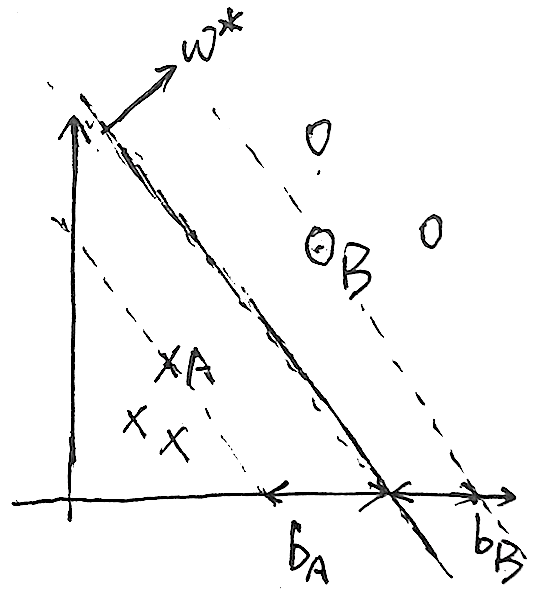
\includegraphics[width=0.5\textwidth]{./images/b}
  \caption{Intercept illustration for $b$ calculation: calculate the $b_A,b_B$ the closest "b" to the plane from either side, then infer $b$ from these tow values.}\label{fig:b}
\end{figure}
\textbf{Recover $w,b$ from $\alpha$-s}. Assuming we have solved the dual problem (next section) and we have the solution on $\alpha$, let's call it $\alpha^\ast$. Then we can calculate the solution in original parameters, call it $w^\ast$, $b^\ast$ as following:
$$
	w^\ast = \sum_{i=1}^{m} \alpha^\ast y_i x_i 
$$
And as shown in Figure \ref{fig:b}, we can first calculate $b_A$ and $b_B$, then get $b^\ast$:

$b_A = \max_{i:y_i = -1} w^{\ast T} x_i $ This is the maximum on negative points that $b^\ast$ has to compensate to -1: $b^\ast\leq -1-b_A$\\

$b_B = \min_{i:y_i = 1} w^{\ast T} x_i$  This is the minimum on positive points that $b^\ast$ has to compensate to 1: $b^\ast\geq 1-b_B$\\

Will take $b^\ast$ to be the average of these two values: $b^\ast = - \frac{b_A + b_B} {2}$



%%%%%%%%%%%%%%%%%%%%%%%%%%%%%%%%%%%%%%%%%%%%%%%%
\subsection{Kernel trick}
Will be discussing separately kernels, but for now it is worth to point out the kernel trick: We notice that there are many dot products ($x_i^T x_j$) in our formula. We can keep the whole SVM-DUAL setup, and the algorithms for solving these problems, but choose \textbf{kernel function} $k(x_i^T, x_j)$ to replace the dot products ($x_i^T x_j$). To qualify as a kernel, informally, the function $k(x_i,x_j)$ must be a dot product $k(x_i,x_j)$ = $\Phi(x_i)* \Phi(x_j)$, where $\Phi(x)$ is a mapping vector from the original feature space \{$X$\} into a different feature space \{$\Phi(X)$\}.  

The essential ``trick'' is that usually $\Phi$ is not needed or known, only $k(x_i,x_j)$ is computable and used. To see this for the SVM, it is clear that the dual problem is an optimization written in terms of the dot products replaceable with a given kernel $k(x_i,x_j)$. 

How about testing? The parameter  $w = \sum_{i=1}^{m}\alpha_i y_i \Phi(x_i)$ is not directly computable if we dont know explicitly the mapping $\Phi()$, but it turns out we dot need to compute $w$ explicitly; we only need to compute predictions for test points $z$:


 $w\Phi(z)+b = \sum_{i=1}^{m}\alpha_i y_i \Phi(x_i)\Phi(z)+b =\sum_{i=1}^{m}\alpha_i y_i k(x_i,z)+b$\\

This fact has profound implications to the ability of representing data and learning from data: we can apply SVM to separate data which is not linearly separable! Thats because even if the data is not separable in the original space \{$X$\}, it might be separable in the mapped space \{$\Phi(X)$\}. The kernel trick is not specific to SVMs; it works with all algorithms that can be written in terms of dot products $x_i*x_j$.



%%%%%%%%%%%%%%%%%%%%%%%%%%%%%%%%%%%%%%%%%%%%%%
\subsection{Non-Separable case and slack variables}
The derivation of the SVM as presented so far assumed that the data is linearly separable. In some cases, it is not clear that finding a separating hyperplane is exactly what we'd want to do, since that might be susceptible to outliers. For instance, the Figure \ref{fig:outlier}, it causes the decision boundary to make a dramatic swing, and the resulting classifier has a much smaller margin. 
\begin{figure}[h!]
  \centering
    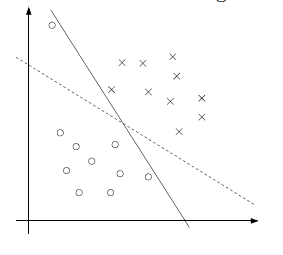
\includegraphics[width=0.5\textwidth]{./images/outlier}
  \caption{Outlier Example}\label{fig:outlier}
\end{figure}

To make the algorithm work for non-linearly separable datasets as well as be less sensitive to outliers, we reformulate the optimization(using $\mathcal{L}_1 \quad regularization$) as following:
\begin{align*}
& \min_{w, b, \xi} \frac{1}{2} ||w||^2 + C \sum_{i=1}^{m}\xi_i\\
	\text{s.t.}  &\quad y_i (w^T x_i + b) \geq 1 - \xi_i, \quad i = 1, \dots, m \\
	& \quad \xi_i \geq 0, \quad i = 1, \dots, m  
\end{align*}
Thus, examples are now permitted to have margin less than 1, and if an example has functional margin $1-\xi_i$ (with $\xi > 0$), we would pay a cost of the objective function being increased by $C\xi_i$. The parameter $C$ controls the relative weighting between the twin goals of making the $||w||^2$ small and of ensuring that most examples have functional margin at least 1.\\

\textbf{SVM-DUAL FORM with SLACK VARIABLES}
\begin{align}
	\max_{\alpha} W(\alpha) &= \sum_{i=1}^{m} \alpha_i - \frac{1}{2} \sum_{i,j=1}^{m} y_i y_j \alpha_i \alpha_j x_i^T x_j	\\
		\text{s.t.} \quad & 0 \leq \alpha_i \leq C, \quad, i = 1, \dots, m \nonumber \\
		& \sum_{i=1}^{m} \alpha_i y{(i)} = 0. \nonumber
\end{align}
In adding $\mathcal{L}_1 \quad regularization$, the only change to the dual problem is that was originally a constraint that $0 \leq \alpha_i$ has now become $0 \leq \alpha_i \leq C$. The calculation for $w^\ast$ is the same way, but the calculation for $b^\ast$ has to be modified ($b^\ast$ calculation discussed as part of SMO solver). In this case there are three types of training points
\begin {itemize}
\item $\alpha=0$: non interesting points
 \item $C>\alpha>0; \beta=0$:  a support vector on the margin line, no slack variable; \quad $y_i (w^T x_i + b) = 1$, $\xi_i=0$
 \item $\alpha=C; \beta>0$: a support vector, inside the side (or even misclassified): $\xi_i>0$; $y_i (w^T x_i + b) < 1$, $\xi_i>0$
\end{itemize}


%%%%%%%%%%%%%%%%%%%%%%%%%%%%%%%%%%%%%%%%%%%%%%
\subsubsection {Slack variables dual form derivation [optional material]}
Let's derive this non-separable problem like we did before. We will have additional constrains for slack variables $ \xi_i\geq0$

\begin{enumerate}
\item{Non-separable problem
\begin{align*}
	& \min_{w, b, \xi} \frac{1}{2} ||w||^2 + C \sum_{i=1}^{m}\xi_i\\
	\text{s.t.}  &\quad y_i (w^T x_i + b) \geq 1 - \xi_i, \quad i = 1, \dots, m \\
	& \quad \xi_i \geq 0, \quad i = 1, \dots, m  
\end{align*}}

\item{Constraint transformed: 
	\begin{align*}
	g_i (w, b) = 1- \xi_i -y_i (w^T x_i + b) \leq 0 \\
	h_i (w, b) = - \xi_i \leq 0
	\end{align*}
}

\item{Lagrangian: 
$$\mathcal{L}(w, b, \xi, \alpha, r) = \frac{1}{2} ||w||^2 + C \sum_{i=1}^{m}\xi_i - \sum_{i=1}^{m}\alpha_i (y_i(w^T x_i +b) + \xi_i - 1) - \sum_{i=1}^{m}r_i \xi_i$$} 

\item{Set $\theta_{\mathcal{D}}(\alpha, r) = \min_{w, b} \mathcal{L}(w, b, \xi, \alpha, r)$} \\
	Derivate $\mathcal{L}$ with respect to $w, b, \xi$ to zero:
	\begin{itemize}
		\item {For $w$: 
		\begin{align}
			&\frac{\partial}{\partial w}\mathcal{L}(w, b, \xi, \alpha, r) = w - \sum_{i=1}^{m}\alpha_i y_i x_i = 0 \nonumber \\ 
			\implies & w = \sum_{i=1}^{m}\alpha_i y_i x_i 
		\end{align}}
		\item {For $b$:
		\begin{align}
			&\frac{\partial}{\partial b}\mathcal{L}(w, b, \xi, \alpha, r) = 0 - \sum_{i=1}^{m}\alpha_i y_i = 0 \nonumber \\
			\implies & \sum_{i=1}^{m}\alpha_i y_i = 0 
		\end{align}}
		\item { For $\xi$:
		\begin{align}
			&\frac{\partial}{\partial \xi}\mathcal{L}(w, b, \xi, \alpha, r) = C - \sum_{i=1}^{m} \alpha_i - \sum_{i=1}^{m} r_i = 0 \nonumber \\
			\implies & C = \sum_{i=1}^{m} \alpha_i + \sum_{i=1}^{m} r_i 
		\end{align}
		}
	\end{itemize}

\item{Put the last three equalities back into $\mathcal{L}$, allows for an objective like before only in lagrangian variables $\alpha$:
	\begin{align}
		\mathcal{L} (w, b, \alpha) &=  \frac{1}{2} ||w||^2 + C \sum_{i=1}^{m}\xi_i - \sum_{i=1}^{m}\alpha_i (y_i(w^T x_i +b) + \xi_i - 1) - \sum_{i=1}^{m}r_i \xi_i \nonumber \\
		&= \frac{1}{2} ||w||^2 + \sum_{i=1}^{m} \alpha_i  \xi_i+ \sum_{i=1}^{m} r_i \xi_i - \sum_{i=1}^{m}\alpha_i (y_i(w^T x_i +b) - 1) - \sum_{i=1}^{m} \alpha_i  \xi_i - \sum_{i=1}^{m} r_i \xi_i\nonumber \\
		&=\frac{1}{2} ||w||^2 - \sum_{i=1}^{m}\alpha_i (y_i(w^T x_i +b) - 1)  \nonumber \\
		&= \frac{1}{2} \sum_{i,j=1}^{m}\alpha_i \alpha_j y_i y_j x_i^T x_j - \sum_{i,j=1}^{m}\alpha_i \alpha_j y_i y_j x_i^T x_j - \sum_{i=1}^{m} \alpha_i y_i b + \sum_{i=1}^{m} \alpha_i \nonumber \\
		&=  \sum_{i=1}^{m} \alpha_i - \frac{1}{2} \sum_{i,j=1}^{m} y_i y_j \alpha_i \alpha_j x_i^T x_j
	\end{align}
	Now we get (15), which is the same with (10) in previous derivatives. Although we added more parameters, we only have $\alpha$ now.
}


\end{enumerate}






%%%%%%%%%%%%%%%%%%%%%%%%%%%%%%%%%%%%%%%%%%%%%%%%%%%%%%%%%%%%%%%%%%%%%%%%%%%%%%%%%%%%%%%%%%%%%%%%
\section{Solution part 2 : SMO Algorithm instead of Quadratic Solvers}
Given the final dual form problem, our goal is to optimize the objective function by given some constraints. First let's see a simple one, which is solving unconstrained optimization problem. 

\subsection{Coordinate Ascent}
If our goal is just to solve an unconstrained optimization problem:
$$
	\max_\alpha W(\alpha_1, \dots, \alpha_m)
$$
The $W$ here is just some function of the parameters $\alpha$'s. To solve this optimization, the idea is that we only choose one parameter, let's say $\hat{\alpha}_i$, and hold all variables $\alpha$'s except $\alpha_i$. So we can only optimize $W$ with respect to just the parameter $\hat{\alpha}_i$. The algorithms is shown as following:
\begin{align*}
	&\text{Loop until convergence: \{} \\
	& \quad \quad \text{For} \quad i = 1, \dots, m, \{ \\
	& \quad \quad \quad \alpha_i := \arg \max_{\hat{\alpha}_i} W(\alpha_1, \dots, \alpha_{i-1}, \hat{\alpha}_i, \alpha_{i+1}, \dots, \alpha_m) \\
	& \quad \quad \} \\
	&\}
\end{align*}
And here is an example of coordinate ascent in action:
\begin{figure}[h!]
  \centering
    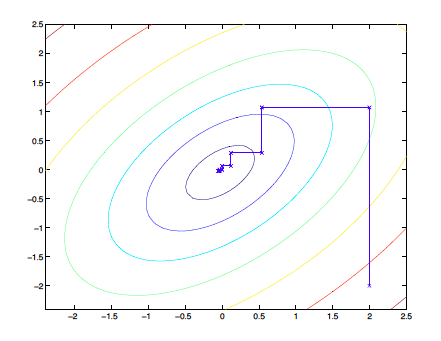
\includegraphics[width=0.7\textwidth]{./images/coordinate}
  \caption{Coordinate Ascent}\label{fig:coordinate}
\end{figure}
Notice that in Coordinate ascent each step, it only takes a step that's parallel to one of the axes, since only one variable is being optimized at a time.

\subsection{SMO}
Our dual optimization problem is:
\begin{align}
	\max_{\alpha} W(\alpha) &= \sum_{i=1}^{m} \alpha_i - \frac{1}{2} \sum_{i,j=1}^{m} y_i y_j \alpha_i \alpha_j x_i^T x_j	\\
		\text{s.t.} \quad & 0 \leq \alpha_i \leq C, \quad, i = 1, \dots, m  \\
		& \sum_{i=1}^{m} \alpha_i y^{(i)} = 0. 
\end{align}

We want to solve this optimization problem and also satisfy the constraints (18-19). If we still choose one parameter, let's say $\alpha_1$, and due to the constraint (19), we get $\alpha_1 = - y_i \sum_{2}^{m} \alpha_i y_i$, which doesn't work, because the $\alpha_1$ is also fixed. So how about we choose two parameters instead of just one? This method turns out to be the basic idea behind SMO:
\begin{align*}
	&\text{Repeat until convergence :} \{ \\
	& \quad \quad \text{select two parameters:}\; \alpha_i, \alpha_{j: j \ne i} \\
	& \quad \quad \text{Optimize} \; W(\alpha) \; \text{with respect to} \; \alpha_i, \alpha_j, \text{holding other parameters fixed.} \\
	&\}
\end{align*}

To know more about the SMO, you can refer the paper written by Platt\footnote{Platt, John (1998), Sequential Minimal Optimization: A Fast Algorithm for Training Support Vector Machines} or the notes from CS 229 in Stanford University\footnote{http://cs229.stanford.edu/materials/smo.pdf}. 

\subsection{SMO Details}
Since we just mentioned that in SMO, there are two main steps: $1)$ select two parameters, $\alpha_i$, and $\alpha_j$; $2)$ optimize $W(\alpha)$ with respect to $\alpha_i$, $\alpha_j$, holding other parameters fixed. In this section, we will give more details about how to deal with these two steps.

\subsubsection{How to Select $\alpha_i$ and $\alpha_j$}
The basic idea is that we want to choose the worst $\alpha_i$ and $\alpha_j$ in each step to modify/correct them to make the biggest progress towards the global maximum. For example in Figure \ref{fig:ex1}, we definitely will choose $P_1$ as the path from point A to G.
\begin{figure}[h!]
  \centering
    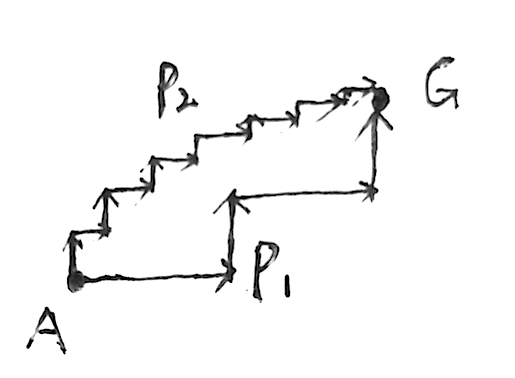
\includegraphics[width=0.7\textwidth]{./images/ex1}
  \caption{Idea about Choosing $\alpha$}\label{fig:ex1}
\end{figure}

So what's the worst $\alpha$? Let's first choose $\alpha_i$ and then $\alpha_j$. 


\begin{itemize}
\item{
\textbf{Selecting $\alpha_i$} \\
The idea about choosing the worst $\alpha_i$ is based on who violates the KKT constrains dual-complementary. Let's recall the KKT dual-complementary(A, B, C, D, E see in Figure \ref{fig:ex2}): 
\begin{figure}[h!]
  \centering
    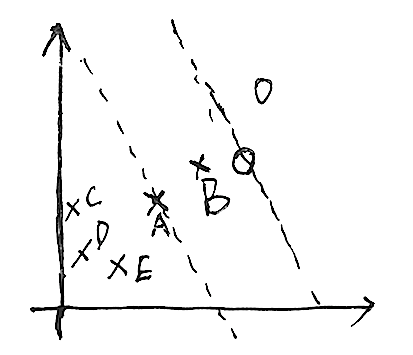
\includegraphics[width=0.7\textwidth]{./images/ex2}
  \caption{KKT dual complementary $\alpha$}\label{fig:ex2}
\end{figure}
\[ KKT \; dual \; complementary: \left\{ 
  		\begin{array}{l l}
			\alpha_i=0 \implies y_if(x_i) \geq 1 & (\xi = 0 \quad \text{correct points, like C,D,E}) \\
			\alpha_i=C \implies y_if(x_i) \leq 1 & (\xi \geq 0 \quad \text{mistake, like B}) \\
			\alpha_i \in (0, C) \implies y_if(x_i)=1 & (\xi=0 \quad \text{support vector, like A})
 		 \end{array} \right.\]

where $f(x_i) = w^T x_i + b$. Thus, violations of KKT is shown as following:
\[ Violations\; of\; KKT \left\{ 
  		\begin{array}{l}
			\alpha_i=0 \; \&\& \; y_if(x_i) < 1 \\
			\alpha_i=C \; \&\& \; y_if(x_i) > 1 \\
			\alpha_i \in (0, C) \; \&\&\; y_if(x_i) \neq 1 
 		 \end{array} \right.\]
}
Let's talk more about the violations of KKT. Why does it violate the KKT? We start from introducing the gap between primal problem and dual problem. We define the gap for a point $(x_i, y_i)$ is:
\begin{align*}
Gap_i &= \alpha_i (y_i(\sum_{j=1}^{m}\alpha_j y_j <x_j, x_i>) - 1) + C\xi_i \\
	  &= \alpha_i (y_i f(x_i) - 1 - y_i b) + C\xi_i \\
\end{align*}
And we also define:
$$
\xi_i = \max(0, 1 - y_i f(x_i))
$$
Let's see each violation of KKT:
\begin{enumerate}
\item{
\begin{align*}
Satisfy:&\\ 
&\alpha_i=0 \&\& y_i f(x_i) \geq 1, \xi=0 \implies  Gap_i^s = 0\\
Violate:& \\ 
&\alpha_i=0 \&\& y_if(x_i) < 1, \xi>0 \implies Gap_i^v =  C\xi_i > Gap_i^s
\end{align*}
}
\item{
\begin{align*}
Satisfy:&\\ 
&\alpha_i=C \&\& y_i f(x_i) \leq 1, \xi=1-y_if(x_i) \implies \\
&Gap_i^s = C(y_if(x_i)-1-y_ib) + C(1-y_if(x_i)) 0 = -Cy_i b \\
Violate:& \\ 
&\alpha_i=C \&\& y_if(x_i) > 1, \xi=0 \implies \\
&Gap_i^v = C(y_if(x_i)-1) - Cy_ib > Gap_i^s
\end{align*}
}
\item{
Easily we can also prove that $Gap_i^v > Gap_i^s$ here.
}
\end{enumerate}
We notice that the gap between primal problem and dual problem will be increased if violating the KKT dual complementary. Thus, we want to choose $\alpha_i$, who violate the KKT, and modify it to reduce the gap. 

Further, we know that there are three violations, which one should we deal first? In fact, in the algorithm, we want to choose all the samples with $\alpha_i \in (0, C)$ first, which are the support vectors. Why? Because non-bound samples have more probabilities to be modified, which means the support vectors effect the hyperplane more than the points, who are not on the hyperplane. After we can not find any non-bound samples, who violate KKT, then we go through the whole samples to check if violating other two KKT dual complementary.

\item{\textbf{Selecting $\alpha_j$}
Select the $\alpha_j$ will follow the rule:
$$
\max_{\alpha_j}|E_i - E_j|
$$
where the $E_i = f(x_i) - y_i$, we will explain why during the later derivation. 
} 
\end{itemize}

\subsubsection{How to Optimize $W(\alpha)$ respect to $\alpha_i$ and $\alpha_j$}
After choosing the $\alpha_i$ and $\alpha_j$, now we would talk about how to optimize the $W(\alpha)$. To make it easy to explain, we set $\alpha_1 = \alpha_i$ and $\alpha_2 = \alpha_j$, we also define:
\begin{align}
&w = \sum_{i=1}^{m}y_i \alpha_i x_i \\
&f(x_i) = w^T x_i + b \\
&K_{i,j} = <x_i, x_j> \quad \text{where using kernel trick} \\
&v_i = \sum_{j=3}^{m} y_j \alpha_j K_{i,j} = f(x_i) - \sum_{j=1}^{2} y_j \alpha_j K_{i,j} - b \\
&E_i = f(x_i) - y_i \\ 
&\eta = K_{i,i} + K_{j,j} - 2K_{i,j} = || \phi(x_i) - \phi(x_j)||^2 
\end{align}

\begin{enumerate}
\item{ \textbf{Calculate $\alpha_j$} \\
First, put $\alpha_1$ and $\alpha_2$ to objective function: \\
\begin{align*}
W(\alpha) &= \sum_{i=1}^{m} \alpha_i - \frac{1}{2} \sum_{i,j=1}^{m} y_i y_j \alpha_i \alpha_j x_i^T x_j \\
		&= \alpha_1 + \alpha_2 + \sum_{i=3}^{m} \alpha_i - \frac{1}{2} \sum_{i=1}^{m} (\sum_{j=1}^{2} y_i y_j \alpha_i \alpha_j K_{i,j} + \sum_{j=3}^{m} y_i y_j \alpha_i \alpha_j K_{i,j})  \\
		&= \alpha_1 + \alpha_2 + \sum_{i=3}^{m} \alpha_i - \frac{1}{2} \sum_{i=1}^{2} (\sum_{j=1}^{2} y_i y_j \alpha_i \alpha_j K_{i,j} + \sum_{j=3}^{m} y_i y_j \alpha_i \alpha_j K_{i,j})  \\ & \quad   \quad  \quad \quad  \quad  \quad \quad \quad - \frac{1}{2} \sum_{i=2}^{m} (\sum_{j=1}^{2} y_i y_j \alpha_i \alpha_j K_{i,j} + \sum_{j=3}^{m} y_i y_j \alpha_i \alpha_j K_{i,j})  \\
		&= \alpha_1 + \alpha_2 + \sum_{i=3}^{m} \alpha_i - \frac{1}{2} \sum_{i=1}^{2} \sum_{j=1}^{2} y_i y_j \alpha_i \alpha_j K_{i,j} - \frac{1}{2} \sum_{i=1}^{2} \sum_{j=3}^{m} y_i y_j \alpha_i \alpha_j K_{i,j}  \\ 
		&  \quad   \quad  \quad \quad  \quad  \quad \quad \quad - \frac{1}{2} \sum_{i=3}^{m} \sum_{j=1}^{2} y_i y_j \alpha_i \alpha_j K_{i,j}  - \frac{1}{2} \sum_{i=3}^{m} \sum_{j=3}^{m} y_i y_j \alpha_i \alpha_j K_{i,j} \\
		&=  \alpha_1 + \alpha_2 + \sum_{i=3}^{m} \alpha_i - \frac{1}{2} y_1^2 \alpha_1^2 K_{1,1} - \frac{1}{2} y_2^2 \alpha_2^2 K_{2,2} - y_1 y_2 \alpha_1 \alpha_2 K_{1,2} \\ 
		&\quad   \quad  \quad \quad  \quad - y_1\alpha_1 \sum_{j=3}^{m} y_j \alpha_j K_{1,j} - y_2 \alpha_2 \sum_{j=3}^{m} y_j \alpha_j K_{2,j} - \frac{1}{2} \sum_{i=3}^{m} \sum_{j=3}^{m} y_i y_j \alpha_i \alpha_j K_{i,j} \\
		&= \alpha_1 + \alpha_2 -\frac{1}{2}K_{1,1}\alpha_1^2 - \frac{1}{2}K_{2,2}\alpha_2^2 - y_1 y_2 K_{1,2} \alpha_1 \alpha_2 - y_1 \alpha_1 v_1 - y_2 \alpha_2 v_2 + CONSTANT
\end{align*}
In fact, now we can apply two constrains (18) and (19) to solve this problem. \\
\textbf{Constrain (19):} Due to $\sum_{i=1}^{m} \alpha_i y_i = 0$, and $\alpha_3, \dots, \alpha_m$ and $y_3, \dots, y_m$ are fixed, so we can set:
$$
	\alpha_1 y_1 + \alpha_2 y_2 = C'
$$
and we can get
\begin{align*}
	& y_1 (\alpha_1 y_1 + \alpha_2 y_2) = y_1 C' \\
	\implies & \alpha_1 + \alpha_2 y_1 y_2 = y_1 C' \\
	\implies & \alpha_1 = y_1 C' - \alpha_2 y_1 y_2 \quad \text{Set} \;  y_1 C' = \gamma \; \text{and} \;  y_1 y_2 = s \\
	\implies & \alpha_1 = \gamma - \alpha_2 s
\end{align*}
Now put $\alpha_1$ to $W(\alpha)$:
\begin{align*}
W(\alpha) &= \gamma - s \alpha_2 + \alpha_2 -\frac{1}{2}K_{1,1}(\gamma - s\alpha_2)^2 - \frac{1}{2}K_{2,2}\alpha_2^2 - sK_{1,2}(\gamma - s\alpha_2)\alpha_2 \\
	& \quad \quad \quad \quad\quad \quad  - y_1 (\gamma - s\alpha_2) v_1 - y_2 \alpha_2 v_2 + CONSTANT
\end{align*}
And derivate $W(\alpha)$ respect to $\alpha_2$:
\begin{align*}
	\frac{\partial W(\alpha)}{\partial \alpha_2} &= -s + 1 + K_{1,1} s \gamma - K_{1,1} \alpha_2 - K_{2,2} \alpha_2 - s \gamma K_{1,2} + 2K_{1,2}\alpha_2  + y_2 v_1 - y_2 v_2 \\
	&= 0
\end{align*}
Put $s=y_1 y_2$ and $y_2^2 = 1$, we can get:
\begin{align*}
& y_2 (y_2 - y_1 + y_1 \gamma (K_{1,1} - K_{1,2}) + v_1 - v_2) - \alpha_2 (K_{1,1} + K_{2,2} -2K_{1,2}) = 0 \\
\implies & \alpha_2^{new} = \frac{y_2 (y_2 - y_1 + y_1 \gamma (K_{1,1} - K_{1,2}) + v_1 - v_2)}{K_{1,1} + K_{2,2} - 2 K_{1,2}}
\end{align*}
After that, we combine$\gamma = \alpha_1^{old} + s \alpha_2^{old}$, $(24) $and $(25)$ and get:
\begin{align}
&\alpha_2^{new} = \alpha_2^{old} + \frac{y_2 (E_1 - E_2)}{\eta} \nonumber \\
\implies & \alpha_j^{new} = \alpha_j^{old} + \frac{y_j (E_i - E_j)}{\eta}
\end{align} 
\textbf{Constrain (18):} Due to $0 \leq \alpha_i \leq C$, so the $\alpha_2$ and $\alpha_1$ must be into a $(0, C) \times (0, C)$ box, shown in the Figure \ref{fig:constrain}.
\begin{figure}[h!]
  \centering
    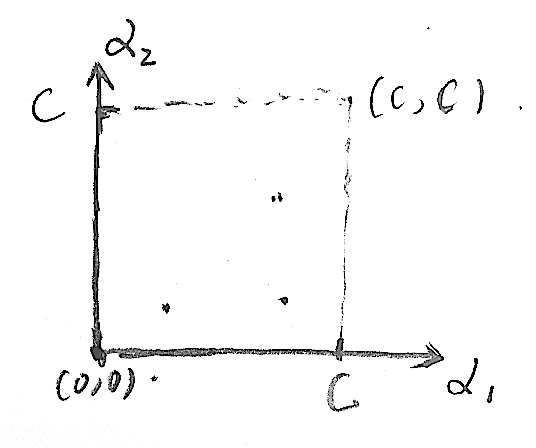
\includegraphics[width=0.7\textwidth]{./images/constrain}
  \caption{Constrains on $\alpha$}\label{fig:constrain}
\end{figure}
And as defined in previous: $\alpha_1 y_1 + \alpha_2 y_2 = C'$.
Now we can consider that there are two different situations: 
\begin{itemize}
	\item{\textbf{if $y_1$, $y_2$ are the same value: [$y_1 y_2 = 1$]}\\
	Then we can get $\alpha_1 + \alpha_2 = C'(or -C' \text{which is the same})$. For example in the Figure \ref{fig:constrains1}, we could get 
	\begin{align*}
		& \alpha_2 \in [0, C] \; \& \; \alpha_2 \in [C' - C, C'] \\
		\implies & \alpha_2 \in [0, C] \; \& \; \alpha_2 \in [\alpha_1 + \alpha_2 - C, \alpha_1 + \alpha_2]
	\end{align*}
	Combine the lower bound and upper bound we could get:
	\begin{align*}
		L_{\alpha_2} &= \max{(0, \alpha_1 + \alpha_2 - C)} \\
		H_{\alpha_2} &= \min{(C, \alpha_1 + \alpha_2)}
	\end{align*}
	\begin{figure}[h!]
 	 \centering
   	 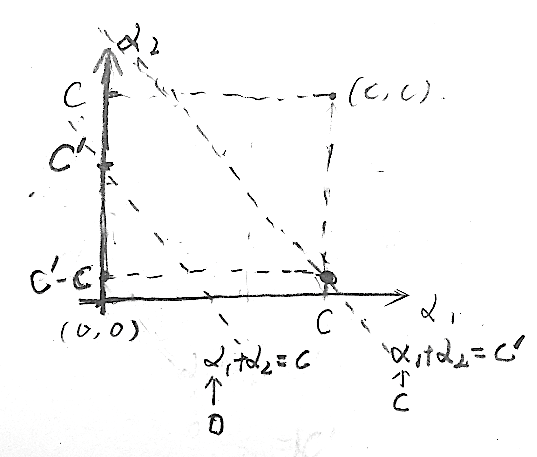
\includegraphics[width=0.7\textwidth]{./images/constrains1}
  	\caption{$y_1, y_2$ same value}\label{fig:constrains1}
	\end{figure}
	}
	\item{\textbf{if $y_1$, $y_2$ are different value: [$y_1 y_2 = -1$]} \\
	Then we could get $\alpha_1 - \alpha_2 = C' (or -C' \text{which is the same})$. For example in the Figure \ref{fig:constrains2}, we could get
	\begin{align*}
		& \alpha_2 \in [0, C] \; \& \; \alpha_2 \in [-C', C-C'] \\
		\implies & \alpha_2 \in [0, C] \; \& \; \alpha_2 \in [\alpha_2 - \alpha_1, \alpha_2 - \alpha_1 + C]
	\end{align*}
	Combine the lower bound and upper bound we could get:
	\begin{align*}
		L_{\alpha_2} &= \max{(0, \alpha_2 - \alpha_1)} \\
		H_{\alpha_2} &= \min{(C, \alpha_2 - \alpha_1 + C)}
	\end{align*}
	\begin{figure}[h!]
 	 \centering
   	 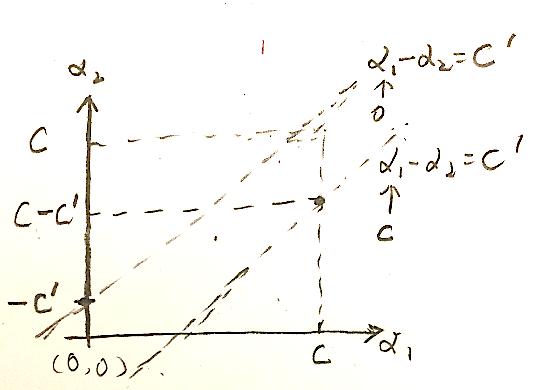
\includegraphics[width=0.7\textwidth]{./images/constrains2}
  	\caption{$y_1, y_2$ different value}\label{fig:constrains2}
	\end{figure}
	} \\
\end{itemize}
Generally:
\begin{align*}
& if \; y_i \neq y_j: L =  \max{(0, \alpha_j - \alpha_i)} \; \text{and} \; H = \min{(C, \alpha_j - \alpha_i + C)} \\
& if \; y_i = y_j: L =  \max{(0, \alpha_i + \alpha_j - C)} \; \text{and} \; H = \min{(C, \alpha_1 + \alpha_2)}
\end{align*}
Then we can use this limitations to clip the $\alpha_j$ like:
\[ \alpha_j^{new,clipped} = \left\{ 
  \begin{array}{l l}
    L & \quad \text{if $\alpha_j^{new} < L$ }\\
    \alpha_j^{new} & \quad \text{if $\alpha_j^{new} \in [L, H] $} \\
    H & \quad \text{if $\alpha_j^{new} > H$}
  \end{array} \right.\]
}

\item{ \textbf{Calculate $\alpha_i$} \\
Once we have got new $\alpha_j$, it won't be hard to calculate $\alpha_i$, notice that we already have:
\begin{align*}
&\alpha_i^{old} = \gamma - s \alpha_j^{old} \\
&\alpha_i^{new} = \gamma - s \alpha_j^{new, clipped} \\
&s = y_i y_j \\
\implies & \alpha_i^{new} = \alpha_i^{old} + s \alpha_i^{old} - s \alpha_j^{new, clipped} \\
& \quad \quad \; = \alpha_i^{old} + y_i y_j (\alpha_j^{old} - \alpha_j^{new, clipped})	 
\end{align*}
}

\item{\textbf{Calculate $b$} \\
When we calculate the bias $b$, we are based on the point whether it's the non-bound points(support vector) or not. (Like point A in Figure \ref{fig:ex2}):
$$
	y_i  f(x_i) = 1.
$$
Now we can divide the situations to four parts:
\begin{itemize}
\item{ \textbf{if only $\alpha_1^{new} \in (0, C)$:} \\
\begin{align*}
& y_1 f(x_1) = 1 \\
\implies & y_1 (\alpha_1^{new} y_1 K_{1,1} + \alpha_2^{new, clipped} y_2 K_{2,1} + \sum_{i=3}^{m}(\alpha_iy_iK_{i,1}) + b_1^{new}) = 1 \\
& E_1 = f(x_1) - y_1 = \alpha_1^{old}y_1 K_{1,1} + \alpha_2^{old} y_2 K_{2,1} + \sum_{i=3}^{m}(\alpha_i y_i K_{i,1}) + b^{old} - y_1 \\
\implies & \sum_{i=3}^{m}(\alpha_i y_i K_{i,1}) = E_1 -  \alpha_1^{old}y_1 K_{1,1} - \alpha_2^{old} y_2 K_{2,1} - b^{old} + y_1 \\
\text{combine them} & \\
\implies &b_i^{new} = b_1^{new} = b^{old} - E_1 + (\alpha_1^{old} - \alpha_1^{new})y_1K_{1,1} + (\alpha_2^{old} - \alpha_1^{new})y_2 K_{2,1} 
\end{align*}
}
\item{ \textbf{if only $\alpha_2^{new} \in (0,C)$:} \\
Same thing we could get
$$
b_j^{new} = b_2^{new} = b^{old} - E_2 + (\alpha_1^{old} - \alpha_1^{new})y_1K_{1,1} + (\alpha_2^{old} - \alpha_1^{new})y_2 K_{2,1} 
$$
}

\item{ \textbf{if both are non-bound:} \\
Choose one of $b_1^{new}$ or $b_2^{new}$.
}

\item{ \textbf{if both are not non-bound:} \\
We choose could set $b^{new}$ as:
$$
b^{new} = \frac{b_1^{new} + b_2^{new}} {2}
$$
}
\end{itemize}
Generally, we update $b$ as:
\[ b^{new} = \left\{ 
  \begin{array}{l l}
    b_i^{new} & \quad \text{if $\alpha_i^{new} \in (0, C)$ }\\
    b_j^{new} & \quad \text{if $\alpha_j^{new, clipped} \in (0, C) $} \\
    \frac{b_i^{new}+b_j^{new}}{2} & \quad \text{otherwise}
  \end{array} \right.\]
}
\end{enumerate}

\subsubsection{SMO Pseudocode}
Now we hope you get a clear idea about how to implement the SMO code. Here is a pseudo code, which is exactly following above derivation steps, and it works in practice. 

For the pseudo code, there are two loops: outer loop and inner loop. In outer loop, we choose $\alpha_i$ and in the inner loop, we update the parameters.
\begin{align*}
\text{Outer loop}&\text{(Choose $\alpha_i$):} \\
	& \text{1) Prefer find $\alpha_i$, who is $0 \leq \alpha_i \leq C$, non-boundary samples.}\\
	& \text{2) If cannot find any samples above, we go through all other data samples.} \\
\text{Inner loop}&\text{(Update parameters):} \\
&\text{1) First check if $\alpha_i$ violates the KKT 	dual complementary }\\
&\text{2) If $\alpha_i$ violates KKT:} \\
& \quad \text{we updating as following steps:} \\
& \quad \quad \text{Step 1: Choose j, by rule:} \max_{\alpha_j}|E_i - E_j| \\
& \quad \quad \text{Step 2: Calculate H, L based on if } y_i = y_j: \\
& \quad \quad \quad \quad \quad \quad \quad \text{if $H == L$, return $0$} \\
& \quad \quad \text{Step 3: Calculate } \eta: \\
& \quad \quad \quad \quad \quad \quad \quad \text{if $\eta \leq 0$, return $0$} \\
& \quad \quad \text{Step 4: Calculate } \alpha_j^{new} \\
& \quad \quad \text{Step 5: Chip } \alpha_j^{new, chipped } \\
& \quad \quad \text{Step 6: Check step distance = } |\alpha_j^{old} - \alpha_j^{new,chipped}|: \\
& \quad \quad \quad \quad \quad \quad \quad \text{if step distance $\leq \epsilon$, return $0$} \\
& \quad \quad \text{Step 7: Update } \alpha_i^{new} \\
& \quad \quad \text{Step 8: Update b}.
\end{align*}


%%%%%%%%%%%%%%%%%%%%%%%%%%%%%%%%%%%%%%%%%%%%%%%%%%%%%%%%%%%%%%%%%%%%%%%%%%%%%%%%%%%%%%%%%%%%%%%%
\section{Lagrange Duality [optional material]}

As mentioned before, the problem is solving constrained optimization problems. In fact, we are familiar with the problem of optimization without any constrains, we can consider gradient descent, Newtown's method, interval cutting etc. Before solving the constrained optimization problems, we need talk about the Lagrangian, Primal and Dual problems.

\subsection{Lagrange}
Lagrange multipliers to solve the problem of the following form, whose constrain is an equality:
\begin{align*}
&\quad \min_{w} f(w) \\
&\quad \text{s.t.} \quad  h_{i}(w) = 0, \quad i = 1, \dots,l
\end{align*}

We can use Lagrange multipliers on it. And in this method, we define the Lagrangian as following:
$$
	\mathcal{L} (w, \beta) = f(w) + \sum_{i=1}^{l} \beta_i h_i(w)
$$

We would find and set $\mathcal{L}$'s partial derivatives to zero:
$$
	\frac{\partial \mathcal{L}}{\partial w_i} = 0; \quad \frac{\partial \mathcal{L}}{\partial \beta_i} = 0
$$

And then we can get the $w^\ast$ to be the solution from the partial derivatives step.

\subsection{Primal Problem}
Consider the following, which we will call the primal optimization problems, whose has inequality as well as equality constraints. 
\begin{align*}
	&\min_w f(w) \\
	\quad  \text{s.t.} &\quad g_i(w) \leq 0, \quad i = 1, \dots, k \\
	\quad &\quad f_i(w) = 0, \quad i = 1, \dots, l.
\end{align*}

Then we can define the generalized Lagrangian
$$
	\mathcal{L}(w, \alpha, \beta) = f(w) + \sum_{i=1}^{k} \alpha_i g_i(w) + \sum_{i=1}^{l} \beta_i h_i(w)
$$

Here consider the quantity
$$
	\theta_{\mathcal{P}}(w) = \max_{\alpha, \beta : \alpha_i \geq 0} \mathcal{L}(w, \alpha, \beta)
$$

In the problem $\theta_{\mathcal{P}}(w)$, if $g_i(w) > 0$ or $f_i(w) \ne 0$, which violates any of the primal constraints given above, then you should be able to verify that 
\begin{align*}
	\theta_{\mathcal{P}}(w) &= \max_{\alpha, \beta : \alpha_i \geq 0} f(w) + \sum_{i=1}^{k} \alpha_i g_i(w) + \sum_{i=1}^{l} \beta_i h_i(w) \\
	&= \infty
\end{align*}

Conversely, if the constraints are indeed satisfied for a particular value of $w$, then $\theta_{\mathcal{P}}(w) = f(w)$. Hence,
	\[ \theta_{\mathcal{P}}(w) = \left\{ 
  		\begin{array}{l l}
    			f(w) & \quad \text{if $w$ satisfies primal constraints}\\
 			\infty & \quad \text{otherwise}
 		 \end{array} \right.\]

Thus, $\theta_{\mathcal{P}}$ takes the same value as the objective in our problem for all values of $w$ that satisfies the primal constraints, and is positive infinity if the constraints are violated. Hence the minimization problem has been transformed to
$$
	\min_{w} \theta_{\mathcal{P}}(w) = \min_{w}  \max_{\alpha, \beta : \alpha_i \geq 0} \mathcal{L}(w, \alpha, \beta)
$$

For later use, we define $p^\ast = \min_w \theta_{\mathcal{P}}(w)$ as the value of the primal problem. In fact, we see that primal problem has the same solutions as our original problem. 

\subsection{Dual Problem}
Then we can define
$$
	\theta_{\mathcal{D}} (\alpha, \beta) = \min_{w} \mathcal{L} (w, \alpha, \beta)
$$
and then pose the dual optimization problem:
$$
	\max_{\alpha, \beta : \alpha \geq 0} \theta_{\mathcal{D}}(\alpha, \beta) = \max_{\alpha, \beta : \alpha \geq 0} \min_{w} \mathcal{L} (w, \alpha, \beta)
$$
And we also define $d^\ast=\max_{\alpha, \beta : \alpha \geq 0} \theta_{\mathcal{D}}(\alpha, \beta) $. We can see that dual problem is pretty similar to our primal problem shown above, except that the order of the ``max'' and the ``min'' are now exchanged.


\begin{figure}[h!]
  \centering
    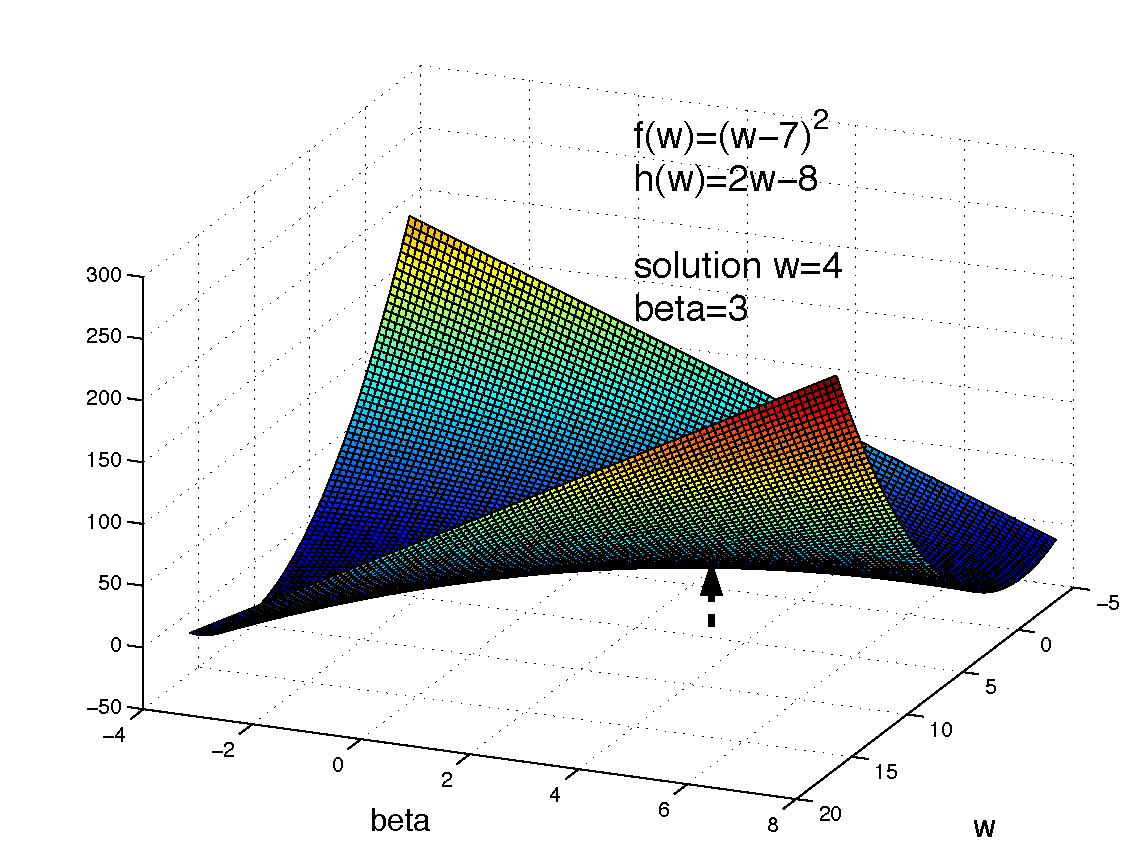
\includegraphics[width=\textwidth]{./images/lagrangian_eq_saddle_beta}
  \caption{Saddle Point}\label{fig:saddle}
\end{figure}
For problem with convex objectives and linear constraints the \textbf{duality gap always closes} (KKT theorem) in the sense that  

$\max_{\alpha, \beta : \alpha \geq 0} \min_{w} \mathcal{L} (w, \alpha, \beta) = \min_{w}  \max_{\alpha, \beta : \alpha_i \geq 0} \mathcal{L}(w, \alpha, \beta)$\\

 The solution is exactly this "saddle point" : maximum of the minimums of each convex slice, same as minimum of the maximums of each concave slice (shown in Figure\ref{fig:saddle}. 




\subsection{Karush-Kuhn-Tucker conditions for duality gap }
How are the primal and the dual problems related? And why should we introduce primal and dual problems? We will talk a little bit in this section. Let's start with why. Since we present our original problem as following:
\begin{align*}
	& \max_{w, b} \frac{1}{2} ||w||^2 \\
	\quad & \text{s.t.} \quad y_i (w^T x_i + b) \geq 1, \quad i = 1, \dots, m
\end{align*}
By introducing Lagrange multipliers $\alpha$, the original constrained problem can be expressed as a primal problem:
\begin{align*}
	w^\ast, b^\ast &= \arg p^\ast = \arg \min_{w, b}\theta_{\mathcal{P}}(w, b) \\
	&= \arg \min_{w, b} \max_{\alpha \geq 0} (\frac{1}{2} ||w||^2 - \sum_{i=1}^{m}\alpha_i (y_i(w^T x_i +b) - 1))
\end{align*}
this is a saddle point\footnote{http://en.wikipedia.org/wiki/Saddle\_point}. If we want to solve this primal problem, we can use QP, which is inefficient. We try to transform the primal problem to the dual problem as following\footnote{http://en.wikipedia.org/wiki/Support\_vector\_machine}:
\begin{align*}
	\alpha^\ast &= \arg d^\ast = \arg \max_{\alpha} \theta_{\mathcal{D}} (\alpha) \\
		&= \arg \max_{\alpha} (\sum_{i=1}^{m}\alpha_i - \frac{1}{2}\sum_{i,j=1}^{m}\alpha_i \alpha_j y_i y_j x_i^T x_j) \\ 
		\text{s.t.} \quad & \alpha_i \geq 0 \\
		\quad & \sum_{i=0}^{m} \alpha_i y_i = 0
\end{align*}
In dual problem, we get rid off two parameters $w, b$ and the constrains are much easier than before. BTW, notice that we have $x_i^T x_j$ in the formula, which gives us a chance apply kernel trick on it. We will talk about it later. 

We can notice that the dual problem is much better than primal problem. If we can transform the original problem to primal problem, and then to dual problem, it will be good steps to the solutions. In fact, the there is some relationship between primal and dual problems. Notice a fact that $\max \min (f) \leq \min \max (f)$, thus
$$
d^\ast = \max_{\alpha, \beta : \alpha \geq 0} \min_{w} \mathcal{L} (w, \alpha, \beta) \leq \min_{w}  \max_{\alpha, \beta : \alpha_i \geq 0} \mathcal{L}(w, \alpha, \beta) = p^\ast
$$
That's $d^\ast \leq p^\ast$. Further, $d^\ast = p^\ast$ under the KKT conditions.
Once the Primal problem and Dual problem equal to each other, the parameters will meet the KKT conditions. We just introduce the five conditions as following:
\begin{align}
	\frac{\partial}{\partial w_i} \mathcal{L}(w^\ast, \alpha ^ \ast, \beta^\ast) = 0, \quad i = 1, \dots, n \\
	\frac{\partial}{\partial \beta_i} \mathcal{L}(w^\ast, \alpha ^ \ast, \beta^\ast) = 0, \quad i = 1, \dots, l \\
	\alpha_{i}^\ast g_i(w^\ast) = 0, \quad i = 1, \dots, k \\
	g_i(w^\ast) \leq 0, \quad i = 1, \dots, k \\
	\alpha^\ast \geq 0, \quad i = 1, \dots, k 
\end{align}
Later, we will just apply KKT conditions on primal problem to get the dual form problem. 


\end{document}